\chapter{Requisiti soddisfatti}
In questo capitolo vengono illustrati attraverso grafici a torta e tabelle i requisiti funzionali che sono stati implementati all'interno della demo sviluppata per la \textit{Revisione di qualifica}. Utilizzando la codifica descritta all'interno delle \textit{Norme 3.0.0}.

\section{Tabella requisiti funzionali}
\def\tabularxcolumn#1{m{#1}}
{\rowcolors{2}{RawSienna!90!RawSienna!20}{RawSienna!70!RawSienna!40}

	\begin{center}
		\renewcommand{\arraystretch}{1.4}
		\begin{longtable}{|p{4cm}|p{4cm}|}
			\hline
			\rowcolor{airforceblue}
			\makecell[c]{\textbf{Codice Requisito}} & \makecell[c]{\textbf{Soddisfatto}} \\
			%fase 1
			\hline
			\centering RSFO1  & \makecell[tc]{Soddisfatto} \\
			% \shortstack{Capitolato\\Verbale esterno 17-12-2020}   \\
			\hline
			\centering RSFF2 & \makecell[tc]{Non soddisfatto} \\
			\hline
			\centering RSFO3 & \makecell[tc]{Soddisfatto}  \\
			\hline
			\centering RSFO4 & \makecell[tc]{Soddisfatto}  \\
			\hline
			\centering RSFO4.1 & \makecell[tc]{Soddisfatto}  \\
			\hline
			\centering RSFO4.2  & \makecell[tc]{Soddisfatto}  \\
			%fase 2
			\hline
			\centering RSFO5 & \makecell[tc]{Soddisfatto}  \\
			\hline
			\centering RSFD5.1 & \makecell[tc]{Non soddisfatto}  \\
			\hline
			\centering RSFD6 & \makecell[tc]{Non soddisfatto}  \\
			%fase 3
			\hline
			\centering RSFO7 & \makecell[tc]{Soddisfatto}  \\
			\hline
			\centering RSFO8  &  \makecell[tc]{Soddisfatto} 	\\
			\hline
			\centering RSFO9 &  \makecell[tc]{Soddisfatto} 	\\
			\hline
			\centering RSFO10 &  \makecell[tc]{Soddisfatto} 	\\
			\hline
			\centering RSFO11 &  \makecell[tc]{Soddisfatto} 	\\
			\hline
			\centering RSFF12  &  \makecell[tc]{Non soddisfatto} 	\\
			\hline
			\centering RSFD13 &  \makecell[tc]{Non soddisfatto} 	\\
			\hline
			\centering RSFD14  &  \makecell[tc]{Non soddisfatto} 	\\
			\hline
			\centering RSFF15 &  \makecell[tc]{Non soddisfatto} 	\\
			\hline
			\centering RSFF16 &  \makecell[tc]{Non soddisfatto} 	\\
			\hline
			\centering RSFO17 & \makecell[tc]{Soddisfatto} \\
			\hline
			\centering RSFO18 &  \makecell[tc]{Soddisfatto} \\
			\hline
			\centering RSFO18.1 & \makecell[tc]{Soddisfatto} \\
			\hline
			\centering RSFO19 & \makecell[tc]{Soddisfatto} \\
			\hline
			\centering RSFO20 & \makecell[tc]{Soddisfatto} \\
			\hline
			\centering RSFO21 & \makecell[tc]{Soddisfatto} \\
			\hline
			\centering RSFO22  & \makecell[tc]{Soddisfatto} \\
			\hline
			\centering RSFO22.1  & \makecell[tc]{Soddisfatto} \\
			\hline
			\centering RSFO22.2  & \makecell[tc]{Soddisfatto} \\
			\hline
			\centering RSFF23 & \makecell[tc]{Soddisfatto} \\
			\hline
			\centering RSFO24 & \makecell[tc]{Soddisfatto} \\
			\hline
			\centering RSFO25 & \makecell[tc]{Soddisfatto} \\
			\hline
			\centering RSFO26 & \makecell[tc]{Soddisfatto} \\
			\hline
			\centering RSFO27 & \makecell[tc]{Soddisfatto} \\
			\hline
			\centering RSFO28 & \makecell[tc]{Soddisfatto} \\
			\hline
			\centering RSFD29 & \makecell[tc]{Non soddisfatto} \\
			\hline
			\centering RSFO30 & \makecell[tc]{Soddisfatto} \\
			\hline
			\centering RSFF31 & \makecell[tc]{Non soddisfatto} \\
			\hline
			\centering RSFO32 & \makecell[tc]{Soddisfatto} \\
			\hline
			\centering RSFO32.1 & \makecell[tc]{Soddisfatto} \\
			\hline
			\centering RSFO32.1.1 & \makecell[tc]{Soddisfatto} \\
			\hline
			\centering RSFO32.1.2 & \makecell[tc]{Soddisfatto} \\
			\hline
			\centering RSFO32.1.3 & \makecell[tc]{Soddisfatto} \\
			\hline
			\centering RSFO32.2 & \makecell[tc]{Soddisfatto} \\
			\hline
			\centering RSFD33 & \makecell[tc]{Non soddisfatto} \\
			\hline
			\centering RSFD33.1 & \makecell[tc]{Soddisfatto} \\
			\hline
			\centering RSFD33.2 & \makecell[tc]{Non soddisfatto} \\
			\hline
			\centering RSFD34 & \makecell[tc]{Non soddisfatto} \\
			\hline
			\centering RSFD35 & \makecell[tc]{Non soddisfatto} \\
			\hline
			\centering RSFD36 & \makecell[tc]{Non soddisfatto} \\
			\hline
			\centering RSFD36.1 & \makecell[tc]{Non soddisfatto} \\
			\hline
			\centering RSFD36.2 & \makecell[tc]{Non soddisfatto} \\
			\hline
			\centering RSFD37 & \makecell[tc]{Non soddisfatto} \\
			\hline
			\centering RSFD37.1 & \makecell[tc]{Non soddisfatto} \\
			\hline
			\centering RSFD38 & \makecell[tc]{Non soddisfatto} \\
			\hline
			\centering RSFD39 & \makecell[tc]{Non soddisfatto} \\
			\hline
			\centering RSFD40 & \makecell[tc]{Non soddisfatto} \\
			\hline
			\centering RSFD41 & \makecell[tc]{Soddisfatto} \\
			\hline
			\rowcolor{white}
			\caption[Tabella requisiti funzionali]{Requisiti funzionali soddisfatti}\label{3.1}\\
		\end{longtable}%\captionof{table}{Requisiti funzionali}
\end{center}
\section{Grafici requisiti funzionali}\label{GraficiRequisitiFunzionali}
Nel grafico seguente vengono visualizzati tutti i requisiti funzionali soddisfatti.
\begin{center}
	\begin{figure}[H]
		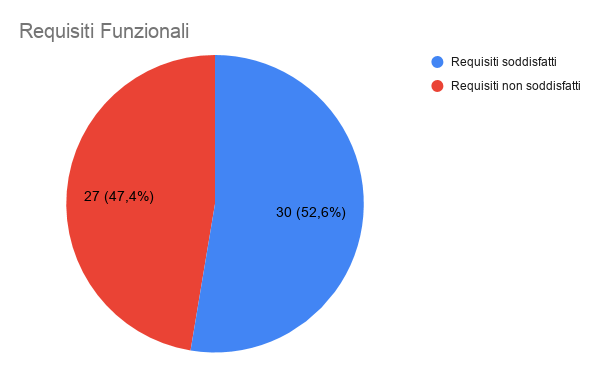
\includegraphics[scale=0.8]{../immagini/diag_PB/torta_RSF.png}
		\caption{Diagramma a torta di tutti i requisiti funzionali soddisfatti}
	\end{figure}
\end{center}

Nel grafico seguente vengono visualizzati tutti i requisiti funzionali obbligatori soddisfatti.

\begin{center}
	\begin{figure}[H]
		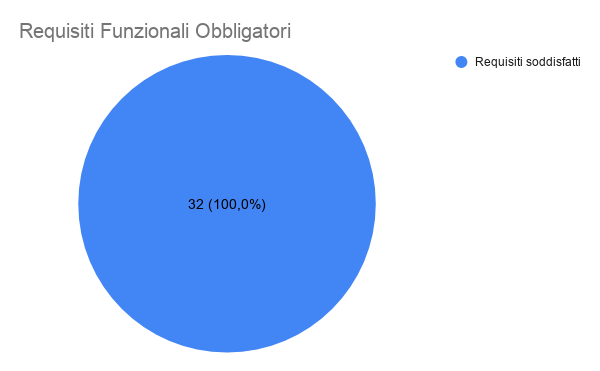
\includegraphics[scale=0.8]{../immagini/diag_PB/torta_RSFO.png}
		\caption{Diagramma a torta di tutti i requisiti funzionali obbligatori soddisfatti}
	\end{figure}
\end{center}
